\documentclass[12pt]{article}
\usepackage[utf8]{inputenc}
\usepackage[a4paper,bottom=2.5cm,left=2cm,right=2cm,top=2cm]{geometry}
\usepackage{soul}

% hyphenation, date format, font encoding
\usepackage[british]{babel}
\usepackage{hardwrap}
\usepackage[T1]{fontenc}
\usepackage{xhfill}

% dagger footnotes & re-start count every page
\usepackage{perpage}
\MakePerPage[2]{footnote}
\renewcommand{\thefootnote}{\fnsymbol{footnote}}

% graphics imports
\usepackage{graphicx}
\usepackage{caption}

% plain page style
\pagestyle{plain}

% conditional page formats
\usepackage{changepage}

% multiple columns & long tables
\usepackage{multicol} \setlength{\columnsep}{3em}
\usepackage{longtable}

% box padding
\setlength{\fboxsep}{1ex}
\renewcommand{\arraystretch}{1.2}

% newlines after packages
\usepackage{parskip}
\setlength{\parskip}{1em}
\makeatletter
\newcommand{\@minipagerestore}{
  \setlength{\parskip}{1em}
}
\makeatother

% lists & tables
\usepackage{enumitem}
\usepackage{multirow}

% puzzle
\usepackage{logicpuzzle}
\usepackage[unboxed]{cwpuzzle}
% fonts & spacing
\usepackage[rm]{roboto}
\usepackage{roboto-mono}
\usepackage{microtype}

% icons
\usepackage{fontawesome}

% alternative font (URW Grotesk)
\newcommand{\altfont}[1]{\fontfamily{ugq}\selectfont \uppercase{#1}}
\renewcommand{\emph}[1]{\textbf{\em{#1}}}

% end mark
\newcommand{\tombstone}[1]{%
  \includegraphics[height=\fontcharht\font`\B,clip]{#1}
}

% title headers
\newcommand{\head}[1]{
  \noindent\xrfill[0.5ex]{0.5pt}\
  \altfont{#1}\
  \xrfill[0.5ex]{0.5pt}
}
\newcommand{\pagehead}[1]{
  \begin{center} {\Huge \head{#1}} \end{center}
  %\vspace{1mm}
}
% smaller header
\newcommand{\subhead}[1]{
  \begin{center}
    \vspace{0.5\baselineskip}
    \parbox{0.95\textwidth}{{\large \head{#1} }}
    \vspace{0.5\baselineskip}
  \end{center}
}


\begin{document}

% TITLE PAGE %
\thispagestyle{empty}
\vspace*{\fill}
        {
          \centering
          
\includegraphics[width=\textwidth,keepaspectratio]
                          {img/picocon39.png}
        }
        \vfill
        \clearpage

        % definition for chair/sofa/beanbag articles
        \newcommand{\seat}[4]{
          % #1 - author name
          % #2 - author post
          % #3 - text source
          % #4 - tombstone
          \vspace{\parskip}
          \input{#3}\tombstone{#4}
          \vspace{0.5\parskip}
          \begin{flushright}
            \parbox{0.4\textwidth}{
              \par {\Large \altfont{#1}}
              \par \vspace{-\parskip} {#2}
            }
          \end{flushright}
        }

        \pagehead{A word from the Chair}
        \seat{Phillip Warburton}{ICSF Entity of Chairs}{txt/chair}{img/t-scifi}
        \vfill
        \newenvironment{smlist}{\begin{itemize}\itemsep-0.6em}{\end{itemize}}
\newcommand{\socialmedia}[2]{
  % #1 - name
  % #2 - address
\item[\raisebox{\dimexpr-.55em}{
    \includegraphics[height=1.6em]{img/media/#1}
}] {\texttt{#2}}
}
\begin{center}
\begin{minipage}{0.25\textwidth}
  \begin{center}
    
\includegraphics[width=0.55\textwidth]{img/media/qr-small}
    \vfill
  \texttt{icsf.org.uk}
  \end{center}
\end{minipage}%
\begin{minipage}{0.3\textwidth}
  \begin{smlist}
  \socialmedia{facebook}{ICSF.Imperial}
  \socialmedia{twitter}{@Picocon}
  \socialmedia{twitter}{@Imperial\_SciFi}
  \socialmedia{instagram}{@Imperial\_SciFi}
  \end{smlist}
\end{minipage}
\end{center}

        \vfill
        \clearpage

        \pagehead{The Sofa's Ramblings}
        \seat{Thomas Blore}{Picocon Sofa}{txt/sofa}{img/t-scifi}

        \pagehead{A Word from the Beanbag}
        \seat{Peter Robson}{Picocon Beanbag}{txt/beanbag}{img/t-scifi}
        \vfill
        \clearpage
        \pagehead{What's On}
        Ah. Once again you find yourself trapped in one of the machinations devised by the Imperial Science Fiction Society --- Picocon. A newcomer, you say? Fear not, for this handbook shall guide you through the perils of the day...

Through the powers of divination and meticulous planning, we shall be graced with the presence of not one, but four, \emph{Guests of Honour}. After lecturing us on the wonders and horrors of these creatures of our design, there shall be a \emph{Guest Panel} where all your questions shall be answered, followed by some book signings. 

After lunch, there shall be righteous \emph{Destruction of Dodgy Merchandise}. The audience (You) shall be given a choice: to save one of these pitiful creations from a fate of total annihilation; or, to bring the hammer of justice (and the cold death of --196 C) down on their stupid little faces. The choice is yours.

In conjunction with this, one shall bear witness to the height of modern chivalry --- \emph{Baguette Bash}. Engage in duels of honour, and destroy your enemies with sticks of rolled bread, or sit on the sidelines and enjoy the show, but only if you are a coward.

The dreaded \emph{Turkey Talks} shall once again be held. Introverts will, for some ineffable reason, willingly choose to speak on stage. The audience shall be given the power to prolong the fool's suffering, in form of charitable donations.

\emph{Imperial Tabletop \& Gaming} will return once more in \emph{Femtocon}. They are cool too, so definitely check out their society as well. As always, those who brave the depths of science fiction and fantasy are always welcome to visit the \emph{Sci-Fi Library}, open lunchtimes throughout the week in Beit's West Basement.

As written.

        \vspace{2.5\baselineskip}
        \pagehead{Tabletop Gaming}
        \seat{Luke Conmy}{\st{ICSF Editor} Head of Boardgames - Tabletop Gaming Society}{txt/gaming}{img/t-gaming}
        \clearpage

        \pagehead{Schedule}
        \begin{calendar}{October}
  \calendarhead
  \calendarweek{
    \calendarday[29]{}
    &\calendarday{\calendarevent{ICSF Library}{Literary Lucky Dip\footnotemark[2]}{}}
    &\calendarday[1]{}
    &\calendarday{\calendarevent{12:00-20:00 ICSF Library}{Wanna-Go Wednesday}{}}
    &\calendarday{\calendarevent{18:00-24:30 Blackett 1004}{Meet and Greet}{}}
    &\calendarday{\calendarevent{}{Themed Friday}{Blockbuster Night}}
    &\calendarday{}
  }
  \calendarweek{
    \calendarday{}
    &\calendarday{}
    &\calendarday{}
    &\calendarday{}
    &\calendarday{}
    &\calendarday{\calendarevent{}{Themed Friday}{Infinity War / Endgame}}
    &\calendarday{}
  }
  \calendarweek{
    \calendarday{}
    &\calendarday{}
    &\calendarday{}
    &\calendarday{\calendarevent{}{EGM\footnotemark[3]}{}}
    &\calendarday{}
    &\calendarday{\calendarevent{}{Cinema Trip}{Zombieland: Double Tap}}
    &\calendarday{}
  }
  \calendarweek{
    \calendarday{}
    &\calendarday{}
    &\calendarday{}
    &\calendarday{}
    &\calendarday{\calendarevent{}{Bar Night}{}}
    &\calendarday{}
    &\calendarday{\calendarevent{}{Book Crawl}{}}
  }
\end{calendar}

\begin{calendar}{November}
  \calendarhead
  \calendarweek{
    \calendarday{}
    &\calendarday{}
    &\calendarday{}
    &\calendarday{}
    &\calendarday{}
    &\calendarday[1]{\calendarevent{18:00-23:00 Dyson Library}{Halloween Party}{}}
    &\calendarday{}
  }
  \calendarweek{
    \calendarday{}
    &\calendarday{}
    &\calendarday{}
    &\calendarday{}
    &\calendarday{}
    &\calendarday{}
    &\calendarday{}
  }
  \calendarweek{
    \calendarday{}
    &\calendarday{}
    &\calendarday{}
    &\calendarday{}
    &\calendarday{}
    &\calendarday{}
    &\calendarday{}
  }
  \calendarweek{
    \calendarday{}
    &\calendarday{}
    &\calendarday{}
    &\calendarday{}
    &\calendarday{}
    &\calendarday{\calendarevent{}{Themed Friday}{Doctor Who}}
    &\calendarday{}
  }
\end{calendar}

\vspace{\fill}

\begin{center}
  \begin{minipage}{0.65\textwidth}
    \itshape
  Regular lunchtime showings (every weekday!) continue throughout
  term-time. Unofficial events not listed.

  More to be announced as we go! Subscribe to our mailing lists to
  receive the latest updates.
\end{minipage}
\end{center}

\vspace{\fill}

        \clearpage

        \pagehead{Guests of Honour}
        \newcommand{\profiletxt}[1]{
  \begin{minipage}[t]{0.74\textwidth}
    \vspace{0pt}
    \input{#1}
  \end{minipage}
}
\newcommand{\profileimg}[2]{
  \begin{minipage}[t]{0.22\textwidth}
    \vspace{0pt}
    \includegraphics[width=\textwidth]{#2}
    \\ [0.5em]
       {\Large \altfont{#1}}
  \end{minipage}
}
\newcommand{\profile}[3]{
  \checkoddpage\ifoddpage
  \profiletxt{#3}\hspace*{\fill}\profileimg{#1}{#2}
  \else
  \profileimg{#1}{#2}\hspace*{\fill}\profiletxt{#3}
  \fi
}
%% \newcommand{\profile}[3]{
%%   % #1 - name
%%   % #2 - path to image
%%   % #3 - path to text
%%   \begin{minipage}[t]{0.74\textwidth}
%%     \vspace{0pt}
%%     \input{#3}
%%   \end{minipage}
%%   \hspace*{\fill}
%%   \begin{minipage}[t]{0.22\textwidth}
%%     \vspace{0pt}
%%     \includegraphics[width=\textwidth]{#2}
%%     \\ [0.5em]
%%     {\Large \altfont{#1}}
%%   \end{minipage}
%% }%
\profile{Brendan Dubois}
        {img/guests/b-dubois.jpg}
        {txt/guests/d-dubois}

\profile{A.J. Flowers}
        {img/guests/a-flowers.jpg}
        {txt/guests/a-flowers}
        
\profile{Louise Mumford}
        {img/guests/l-mumford.jpg}
        {txt/guests/l-mumford}
\profile{Bryony Pearce}
        {img/guests/b-pearce.jpg}
        {txt/guests/b-pearce}
        
\profile{Gareth Powell}
        {img/guests/g-powell.jpeg}
        {txt/guests/g-powell}
        
\profile{Matthew Wraith}
        {img/guests/m-wraith.jpg}
        {txt/guests/m-wraith}

        \clearpage

        \pagehead{Quest Objectives}
        \newcommand{\team}[3]{
  % #1 - name
  % #2 - description
  % #3 - image path
  \hfill
  \begin{minipage}[t]{0.3\textwidth}
    \begin{center}
      \includegraphics[width=0.8\textwidth]{#3}
      \par\vspace{-0.5\baselineskip}
                 {\Large \altfont{#1}}
                 \par\vspace{-0.5\baselineskip}
                 #2
    \end{center}
  \end{minipage}
  \hfill
}

On your way in, you should have been assigned to one of three
teams \textemdash{} \emph{Detective Pikachu}, \emph{Commander Riker},
or \emph{Cthulhu} \textemdash{} and given a sticky badge to
wear with newfound pride. If somehow you slipped through the net, or
misplaced your badge, then go and politely berate the receptionists
until they give you one.

On the next page, you will find a list of dangerous, potentially
impossible items. Find any of these items, bring the evidence back to
the front desk, and win fabulous prizes \ldots in the form of points
for your team. Whichever team ends up with the most points will be
declared the finest, the greatest, and most importantly, the winners!

Now go \emph{for great justice.}

\vspace{1.8\baselineskip}

\begin{center} This year's teams are (drumroll): \end{center}

%\subhead{This year's teams (drumroll):}
\vspace{\baselineskip}

\hfill
\team{The Pikachu\footnotemark[1]}{
  `Pika pika' is the sound of
  \emph{\textasciitilde detective work\textasciitilde} happening.
}{img/quest/pikachu.png}
\team{The Cthulhu\footnotemark[2]}{
  Iä! Iä! Cthulhu fhtagn.}{img/quest/cthulhu.png}
\team{The Rikers}{
  [swings leg over chair and sits down.]}{img/quest/riker.png}
\hfill
%\vspace{1.2\baselineskip}
%\subfoot

\vspace{1.8\baselineskip}

\begin{itemize}[leftmargin=*, itemsep=-0.7\baselineskip]
\item Items can be submitted to the Front Desk for Fun Points™ after 11am.
\item Pictures are (usually) not admissible.
\item Objectives involving people must only be undertaken with the
  person’s permission.
\item The front desk reserves the right to keep the submitted items.
\item Unless otherwise noted, each faction may claim an item on the
  list only once.
\end{itemize}

%(Good luck: you're likely to need it.)

\footnotetext[1]{Pretty sure the plural of Pikachu is still Pikachu.}
\footnotetext[2]{But what is the plural of Cthulhu?}
 \clearpage
        % ugly fix for automatic line-wrapping
\newcommand{\questitem}[2]{
  \texttt{#1} \> \parbox[t]{0.35\textwidth}{#2} \\[0.4\baselineskip]
}
\newcommand{\FD}{\textsuperscript{FD}}
\newcommand{\E}{\textsuperscript{E}}
\newcommand{\M}{\textsuperscript{M}}

\clearpage

\subhead{List of dangerous, potentially impossible items}

\begin{multicols}{2}
  \begin{small}
    \begin{tabbing}
      \hspace*{3.6em} \= \kill
       \questitem{15}     {A Good Cow}
       \questitem{1}     {Hugs (per person)}
       \questitem{10}    {A terrible cosplay~\FD ~\E}
       \questitem{30} {A good cosplay ~\FD ~\E}
       \questitem{50} {A Menagerie-themed cosplay~\FD ~\E}
      \questitem{30}    {Picocon}
      \questitem{20}    {A non-ICSF fresher at Picocon}
      \questitem{Age+5} {Ex-ICSF Chair~\M}
      \questitem{Age+5} {Ex-ICSF Librarian~\M}
      \questitem{Age+5} {Ex-ICSF Treasurer~\M}
      \questitem{Age+5} {Ex-ICSF Editor~\M}
      \questitem{Age+5} {Ex-ICSF Chair of Vice~\M}
      \questitem{Age+5} {Ex-ICSF Secretary~\M}
      \questitem{Age+5} {T-shirts from Picocon's past~\M}
      \questitem{10}    {Previous Guest of Honour~\E}
      \questitem{20}    {Snacks/chocolate for the committee~\FD ~\E}
      \questitem{-15}    {Snacks/chocolate for yourself~\FD ~\E}
      \questitem{10}    {tbh, just any food for the committee ~\E}
     
      \questitem{100}   {The Picocon Sofa, frantic}
      \questitem{50}    {The Picocon Beanbag, calm}
      \questitem{3}    {A good hat ~\FD}
      \questitem{-2}    {A hat with holes}
      \questitem{10} {A portrait of your team mascot.}
       \questitem{15}    {A wizard's pointy hat}
       \questitem{4} {A d20 dice.}
       \questitem{15} {A bowler hat}
       \questitem{45} {A barbershop quartet (+20 points if Menagerie-themed).}
       % \questitem{-30}    {Possession by Chaos}
      \questitem{1000}  {£100~\E}
      % \questitem{7}     {The funniest joke in the world\FD}
      % \questitem{500}     {The One Ring}
      \questitem{2}    {A funny joke~\FD ~\E}
      \questitem{-2}    {A bad pun~\FD ~\E}
      % \questitem{765}    {The Andromeda Galaxy}
      \questitem{30}    {A fairy wand}
      \questitem{15}    {An actual Pokémon}
      \questitem{10}    {Bagpipes}
      \questitem{51} {An alien}
      \questitem{10} {Ten good reasons why Afterlife was awful}
      
      % \questitem{5}     {A Cardboard building\E}
      % \questitem{-5}    {A smashed Cardboard buidling\E}
      \questitem{15}    {2 greek letters}
      % \questitem{50}     {A complete spelling of sci fi with letters from 5 different places}
       \questitem{50}     {A comically large spoon ~\FD}
      % \questitem{5}     {A horde of geese – minimum 3}
       \questitem{20}    {The answers to the quiz – cannot be submitted after half 6}
       \questitem{200}    {A freaking dragon}
       % \questitem{200}      {A unicorn horn}
       \questitem{333}      {A three-headed dog (pettable)}
       \questitem{10} {A UFO}
       
      % \questitem{30}    {Uncle ben}
      % \questitem{100}    {Uncle ben’s corpse}
      % \questitem{33}     {A mourning Peter Parker\E}
      % \questitem{45}     {An object which is bigger on the inside than it is on the outside }
      % \questitem{10}     {The fourth dimension}
      % \questitem{20}     {Even further dimensions \E}
      % \questitem{-1000}    {The novel coronavirus}
      % \questitem{66.7}     {Gravitational lensing}
       \questitem{-20}     {A very awkward moment ~\FD}
      % \questitem{20}     {A functional lightsaber}
      % \questitem{10}    {A working laser blaster}
      % \questitem{5}     {A nanosecond}
      % \questitem{30}    {A bad ghibli movie (impossible)\FD}
      % \questitem{30}    {A terrifying technological terror}
      % \questitem{1}     {The fall of man}
      % \questitem{10}     {Eldritch music}
      \questitem{5}    {A book ICSF lacks (and wants)}
      \questitem{-5}    {A book ICSF lacks (and does not want)}
      \questitem{-10}     {A book ICSF owns (and does not want)}
      % \questitem{30}    {A colour out of space}
      % \questitem{10}    {A fishman}
      \questitem{100} {A menagerie}
      \questitem{-10} {A zombie}
      \questitem{-20} {A ghost}
      \questitem{2}     {Famous first words.}
      \questitem{3}    {Famous last words (subject to checking)}
      \questitem{20}    {Spite}
      \questitem{1} {Had no sleep last night}
      % \questitem{n(n+1)} {A book series with n books\M}
      % \questitem{20}    {The death of innocence}
      % \questitem{20}    {A dragon's real name}
       \questitem{10}    {A healthy obsession}
       \questitem{-10}    {An unhealthy obsession}
       \questitem{5}    {A Worm reference}
       % \questitem{-30}  {Induced scoliosis}
       \questitem{50}     {A thorough, and comprehensible explanation of vorticity to a non-physics/maths student}
       \questitem{15} {Dune popcorn bucket}
       % \questitem{20}   {A curly moustache}
      % \questitem{20}    {An extra - terrestrial}
      % \questitem{40}    {A friendly extra - terrestrial}
      % \questitem{15}    {1 kg Uranium-235 \E}
      % \questitem{15}     {99 kg Uranium 238 \E}
      % \questitem{-10}   {A portal to hell \E}
      % \questitem{10}   {A murderous member of the committee}
      % \questitem{40}   {A non-murderous member of the committee}
      % \questitem{1}    {A survivor\E}
      % \questitem{5}    {A doomsday prepper\E}
      % \questitem{5}     {Horseman of the apocalypse \E}
      % \questitem{15}     {A god of doom and death}
      % \questitem{20}    {A monument to humanity's hubris}
       \questitem{70}    {A lost Doctor Who episode}
      \questitem{3}     {An understood reference~\E}
      \questitem{-3}    {A misunderstood reference~\E}
      \questitem{-10}   {A misunderstood scientific reference~\E}
      \questitem{30}    {A fairy}
       % \questitem{25}    {A shoggoth ~\E}
       \questitem{15}     {A sleeping editor (wake him up(violently))}
       \questitem{25} {A Master Ball.}
       \questitem{5} {Someone who has watched Pantheon.}
       \questitem{50}     {A sandworm}
       \questitem{20}     {Spice Melange}
       \questitem{900} {The current Tech Priest (in person)}
      % \questitem{4}     {The cosmic gears holding our fates in place}
      % \questitem{10}    {True love}
      % \questitem{10}     {True hatred}
      \questitem{-5}    {A fan of a certain ``subgenre'' in the Omegaverse.}
      \questitem{40} {The tentacle of a Kraken} 
       \questitem{15}    {At least three creme eggs.}
       \questitem{150} {At least three phoenix eggs.}
       \questitem{10}     {A doomed time clone}
       \questitem{$\pm$20}      {A justified/unjustified financially irresponsible action ~\FD}
       \questitem{20}       {A bear}
       % \questitem{1000}     {Jonathan Sims}
       \questitem{-10}      {Complaints about Worm references ~\E}
       \questitem{223}      {A reincarnated Archimedes}
       \questitem{15}     {A full reenactment of Duel of the Fates}
       \questitem{5}        {The high ground}
       \questitem{-5}     {Sand}
       \questitem{15} {A sphinx}
       \questitem{5} {A pyramid}
       % \questitem{413}      {A working copy of sburb}
       \questitem{10}  {Rupert's drop}
       \questitem{5}    {A missing board game piece ~\E}
       \questitem{500}      {Dead committee member ~\E}
       \questitem{-70}     {Insanity from exposure to cosmic horror}
       \questitem{60} {Shrek}
       \questitem{40} {Map to Shrek's swamp}
       \questitem{0}     {Proof for Euler's identity}
       \questitem{3}     {Fear}
       \questitem{50} {Name ten dragon types from HTTYD ~\FD ~\M}
       \questitem{125}     {A unicorn}
       \questitem{-30}  {A horse}
       \questitem{5} {Read a story in the fanzine ~\FD ~\E}
       \questitem{5} {A red Poké Ball}
       \questitem{2} {Drinking coffee}
       \questitem{5} {A mythological creature the Editor does not know.}
       % \questitem{1}     {A unicorn}
      \questitem{25}    {The true timeline}
      \questitem{35}    {A fishsword}
      \questitem{35} {A lightsaber}
      \questitem{10} {A copy of Gideon the Ninth for the library.}
      % \questitem{10}    {A gazebo}
      % \questitem{42}     {The answer to life the universe and everything \FD}
      % \questitem{10}     {A good rendition of 'plagues' from Prince of Egypt}
      % \questitem{-10}    {A bad rendition of 'plagues' from Prince of Egypt}
      % \questitem{-50}   {Per fatality}
      % \questitem{10}    {Medium rare human steak}
      % \questitem{5}     {DOOOOOOOOOM}
      % \questitem{3}     {An unobserved tree falling in the woods}
       \questitem{5}     {An Ed ~\E}
       \questitem{10}     {A wild Ed ~\E ~\FD}
       
      % \questitem{5}     {The war of wrath}
      % \questitem{-20}   {Spontaneous combustion whilst dancing~\E}
      % \questitem{5}     {An ajar jar jar jar}
      % \questitem{10}    {Real liquid nitrogen}
      % \questitem{12}    {Simon Pegg}
      \questitem{10}    {A completed nonogram}
      % \questitem{15}    {A completed crossword}
    \end{tabbing}
  \end{small}
\end{multicols}

\vfill

\begin{center}
  \fbox{\parbox{0.8\textwidth}{
    \vspace{0.2\baselineskip}
    \begin{tabular}{ll}
      \FD & Front Desk Person's Discretion\footnotemark\\
      \E  & This item may be claimed multiple times per faction (``each'')\\
      \M  & For each faction, the highest of their scores will be used
    \end{tabular}
    \vspace{0.1\baselineskip}
  }}
\end{center}

\vfill

\footnotetext{
  This actually applies to everything; where it is noted, it indicates
  that you’re unlikely to change anyone's mind with your cunning
  arguments.  }
 \clearpage

        \vfill
        \pagehead{Nonogram}
        \vspace{-1.5em}
\hspace{7em}
\texttt{
  \begin{nonogram}[rows=15,columns=15,scale=0.58,
      fontsize=footnotesize,helplines=5,extracells=3]
    \nonogramV{%
      {1, 1}, {1, 1}, {5, 5}, {1, 1}, {1, 1},
      {1, 1}, {5, 5}, {13}, {3, 3, 3}, {2, 3, 2},
      {2, 3, 2}, {2, 3, 2}, {3, 3, 3}, {13}, {5, 5},
    }
    \nonogramH{%
      {5}, {7}, {1, 3, 3}, {1, 2, 2}, {8, 2},
      {1, 2, 2}, {1, 9}, {7}, {1, 9}, {1, 2, 2},
      {8, 2}, {1, 2, 2}, {1, 3, 3}, {7}, {5},
    }
  \end{nonogram}
}
\begin{center}
\parbox{0.6\textwidth}{\small\textit{Nonogram created by Henry Wild.}}
\end{center}

        \clearpage
        
        \pagehead{Crossword}
        \vfill
\begin{Puzzle}{13}{13}
|[1]C |O |[2]S |M |I    |[3]C |*  |[4]N |A     |V |[5]A |N |[6]I |.
|A    |* |Q    |* |*    |R    |*  |O    |*     |* |B    |* |S    |.
|[7]D |O |U    |B |L    |E    |*  |[8]V |A     |N |D    |A |L    |.
|M    |* |I    |* |*    |E    |*  |I    |*     |* |U    |* |A    |.
|U    |* |R    |* |[9]S |P    |I  |C    |[10]E |* |C    |* |N    |.
|[11]S|L |E    |E |P    |Y    |*  |[12]E|X     |I |T    |E |D    |.
|*    |* |*    |* |A    |*    |*  |*    |T     |* |*    |* |*    |.
|[13]S|P |[14]R|A |W    |[15]L|*  |[16]F|R     |O |[17]Z|E |[18]N|.
|U    |* |A    |* |[19]N|I    |N  |J    |A     |* |O    |* |E    |.
|N    |* |C    |* |*    |S    |*  |O    |*     |* |M    |* |W    |.
|[20]S|P |O    |I |L    |T    |*  |[21]R|U     |B |B    |L |E    |.
|E    |* |O    |* |*    |E    |*  |D    |*     |* |I    |* |S    |.
|[22]T|I |N    |T |I    |N    |*  |[23]S|T     |R |E    |E |T    |.
\end{Puzzle}

\newcommand{\blnk}{\underline{\hspace{2em}}}

\newcommand{\cwclue}[4]{
% #1 - number
% #2 - answer
% #3 - question
% #4 - length
\item[\texttt{#1}] {{#3} ({#4})}
}
\hfill
\begin{minipage}[t]{0.45\textwidth}
\begin{center}{\large \altfont{Across}}\end{center}
\begin{small}
\begin{itemize}[leftmargin=*,topsep=0pt,itemsep=0pt]
\cwclue{ 1}{COSMIC}{The Fantastic Four gained their powers through \blnk rays}{6}
\cwclue{ 4}{NAVANI}{Renowned Brightlady and Artifabrian}{6}
\cwclue{ 7}{DOUBLE}{Prepare for trouble, and make it \blnk}{6}
\cwclue{ 8}{VANDAL}{\blnk Savage, immortal supervillain}{6}
\cwclue{ 9}{SPICE}{The only thing of worth on Arrakis}{5}
\cwclue{11}{SLEEPY}{What the Silmarillion makes most people}{6}
\cwclue{12}{EXITED}{The  Pevensies \blnk our world through a wardrobe}{6}
\cwclue{13}{SPRAWL}{Colloquial name for the setting of \emph{Neuromancer}, \emph{Count Zero} and \emph{Mona Lisa Overdrive}}{6}
\cwclue{16}{FROZEN}{Disney's version of \emph{The Snow Queen}}{6}
\cwclue{19}{NINJA}{Japanese covert agent}{5}
\cwclue{20}{SPOILT}{Joffrey Baratheon in a nutshell}{6}
\cwclue{21}{RUBBLE}{The Vogons turned the Earth to this}{6}
\cwclue{22}{TINTIN}{Belgium's greatest reporter and adventurer}{6}
\cwclue{23}{STREET}{221B Baker \blnk }{6}
\end{itemize}
\end{small}
\end{minipage}
\hfill
\begin{minipage}[t]{0.45\textwidth}
\begin{center}{\large \altfont{Down}}\end{center}
\begin{small}
\begin{itemize}[leftmargin=*,topsep=0pt,itemsep=0pt]
\cwclue{ 1}{CADMUS}{Founder of Thebes and creator of Superboy}{6}
\cwclue{ 2}{SQUIRE}{Podrick Payne was Tyrion Lannister's \blnk in \emph{A Song of Ice and Fire}}{6}
\cwclue{ 3}{CREEPY}{The Uncanny Valley}{6}
\cwclue{ 4}{NOVICE}{A wizard's apprentice}{6}
\cwclue{ 5}{ABDUCT}{What aliens do to cows every other Thursday}{6}
\cwclue{ 6}{ISLAND}{Roke, Azkaban, Númenor}{6}
\cwclue{ 9}{SPAWN}{Star-\blnk of Cthulhu}{5}
\cwclue{10}{EXTRA}{E.T. The \blnk-Terrestrial}{5}
\cwclue{13}{SUNSET}{Tatooine has two of these each day}{6}
\cwclue{14}{RACOON}{Bradley Cooper's Space Rocket}{6}
\cwclue{15}{LISTEN}{Hey! \blnk! : Navi}{6}
\cwclue{16}{FJORDS}{Pining for the \blnk}{6}
\cwclue{17}{ZOMBIE}{Classic Apocalypse}{6}
\cwclue{18}{NEWEST}{Jodie Whittaker is the \blnk Doctor}{6}
\end{itemize}
\end{small}
\end{minipage}
\hfill
\vfill

        \vfill
        \vfill
        \vfill
        \clearpage
        
        \pagehead{A note from the Editor/Advert?}
        \seat{Luke Conmy}{ICSF Editor}{txt/editor}{img/t-scifi}
        
        
        \pagehead{IMPERIAL SCI-FI AND FANTASY SOCIETY MEETS... THE APOCALYPSE}
        \seat{Rebecca Allday}{ICSF Chair of Vice}{txt/poll}{img/t-scifi}
        
        \pagehead{An Elegy for Uncle Ben}
        A loving uncle lost for his good deeds

The light of his grey hair is tainted red

He warned of power and the care it needs

And in the night was shot and left for dead

\centering

\includegraphics[width=0.3\textwidth,keepaspectratio]
{img/ben1.jpg}
        \\
        RIP UNCLE BEN
        
        1952 - 1962/2002/2008/2012/etc.
%%        \thispagestyle{empty}
% there is no esoteric meaning in the strangely specific numbers. It
% was 3AM on the day before printing and I was eyeballing all the
% dimensions.
\vspace*{\fill}

\hspace{\fill}%
\begin{minipage}{\textwidth}
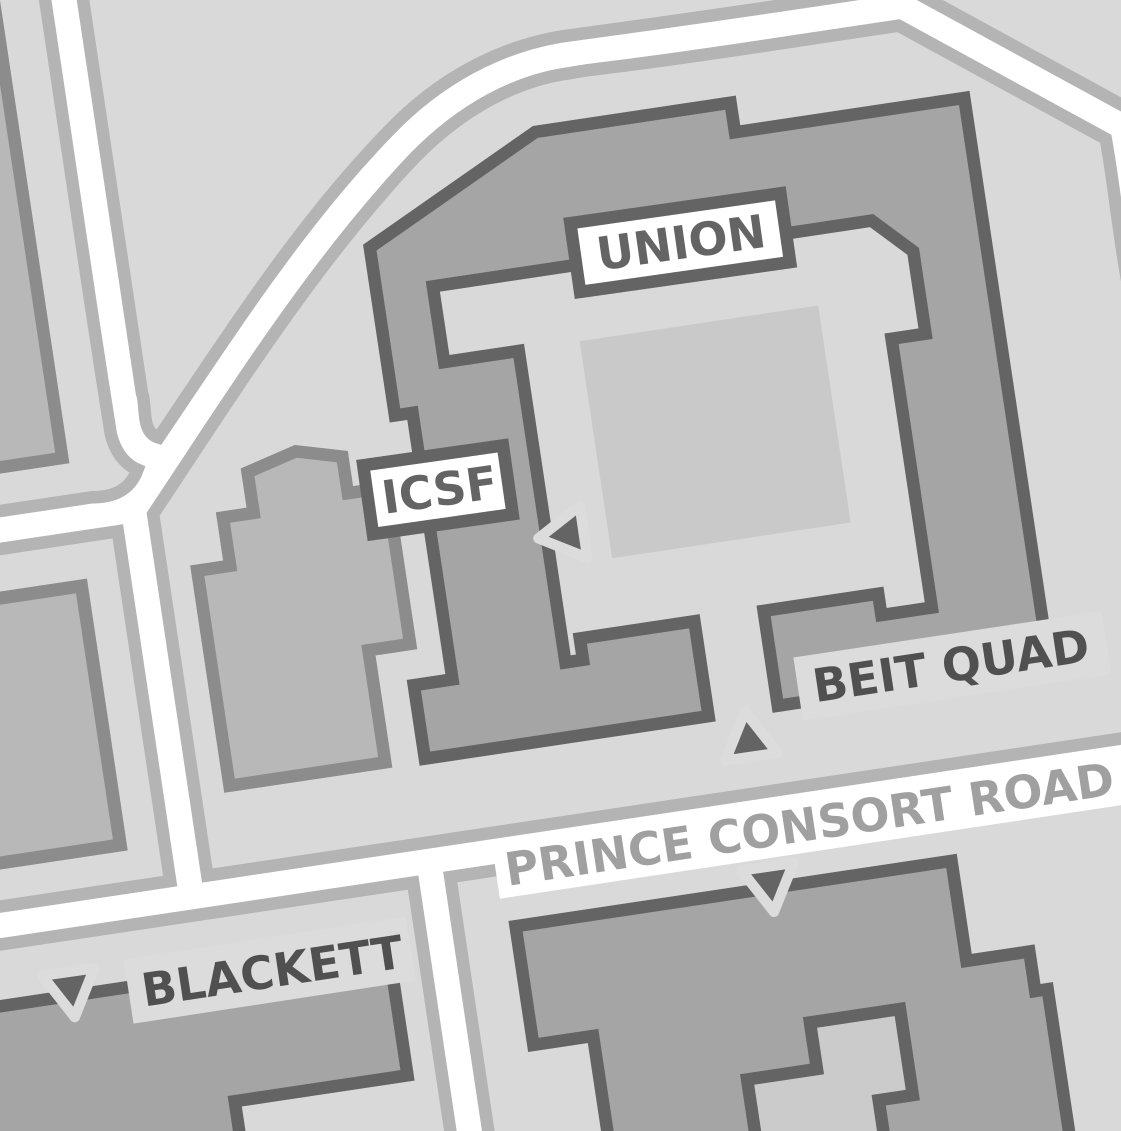
\includegraphics[width=\textwidth]{img/info/map.png}

\vspace{2em}

% QR code for membership
\begin{minipage}[h]{7.8em}

\includegraphics[height=\textwidth]{img/info/qr-small.png}
\end{minipage}%
\hspace{1.5em}%
% logotext
\begin{minipage}[h]{12em}
\raggedright

\includegraphics[width=\textwidth]{img/logo/logo-text.png}
Published November~2023
\texttt{icsf.org.uk}
\end{minipage}
\hspace*{\fill}%
\end{minipage}

        %%        \clearpage
%        \pagehead{Notes and Stuff}
%        \clearpage
\end{document}
